\chapter{Measures}

InVesalius has linear and angular measurements in 2D (axial, coronal and sagittal planes) and 3D (surfaces). It is thus possible to take measurements of volume and area on surfaces.

\section{Linear Measurement}

To perform linear measurements, activate the feature by clicking on the shortcut shown below, located on the toolbar (Figure\ref{fig:measure_line_original}).

\begin{figure}[!htb]
\centering

\includegraphics[scale=0.2]{measure_line_original}
\caption{Shortcut to activate linear measurement}
\label{fig:measure_line_original}
\end{figure}

A linear measurement is taken between two points. With the feature enabled, click \textbf{once} on the image to set the starting point. Then position the mouse pointer on the end point and click once again. The measurement is performed and the result is automatically displayed on the image or surface

Figure~\ref{fig:axial_linear} shows a 2D linear measure in the axial orientation, and Figure~\ref{fig:3d_linear} shows another linear measure in 3D (surface).

Once you have made a 2D linear measurement, it can be edited by placing the mouse on one end, holding down the \textbf{right mouse button} and dragging it to the desired position.

\begin{figure}[!htb]
\centering
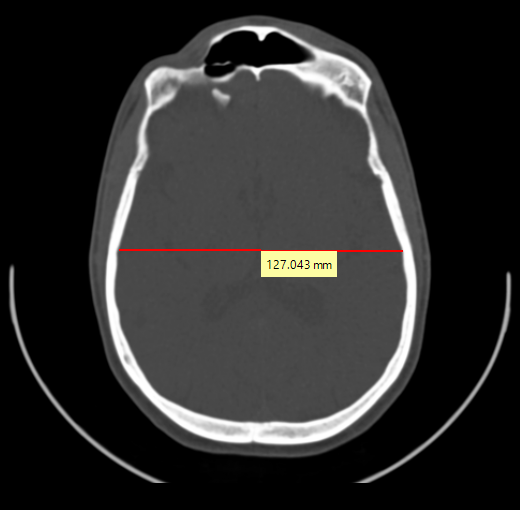
\includegraphics[scale=0.4]{axial_linear.png}
\caption{Linear measure on image}
\label{fig:axial_linear}
\end{figure}

\begin{figure}[!htb]
\centering
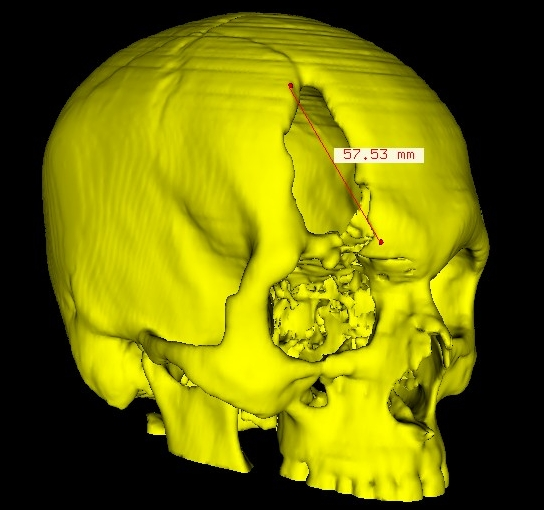
\includegraphics[scale=0.3]{3d_linear.jpg}
\caption{Linear measure on surface}
\label{fig:3d_linear}
\end{figure}

\textbf{Note: The linear measurement is given in millimeters (mm).}

\section{Angular Measurement}

An angular measurement in 2D on a surface (3D) can be done by clicking on the shortcut shown in Figure~\ref{fig:atalho_angular}.

\begin{figure}[!htb]
\centering

\includegraphics[scale=0.2]{measure_angle_original}
\caption{Shortcut for angle measurement}
\label{fig:atalho_angular}
\end{figure}

To perform the angular measurement, it is necessary to provide the three points that will describe the angle to be measured, A\^{B}C. Insert the first point by clicking once to select point A. Insert point B (the vertex or "point" of the angle) by positioning the cursor and clicking once again. Repeat the same actions to determine the endpoint of the angle, C. The resulting measurement is displayed on the image or surface.

Figure~\ref{fig:axial_angular} illustrates an angular measurement on a flat image; Figure~\ref{fig:axial_superficie} illustrates an angular measurement on a surface.

In regards to 2D linear measurement, you can also edit the 2D angular measurement. Just position the mouse on one end, hold down the right mouse button and drag it to the desired position.

\begin{figure}[!htb]
\centering
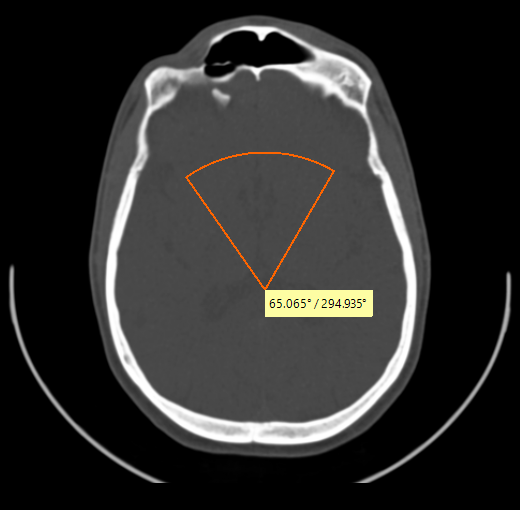
\includegraphics[scale=0.38]{axial_angular.png}
\caption{Angular measurement}
\label{fig:axial_angular}
\end{figure}

\begin{figure}[!htb]
\centering
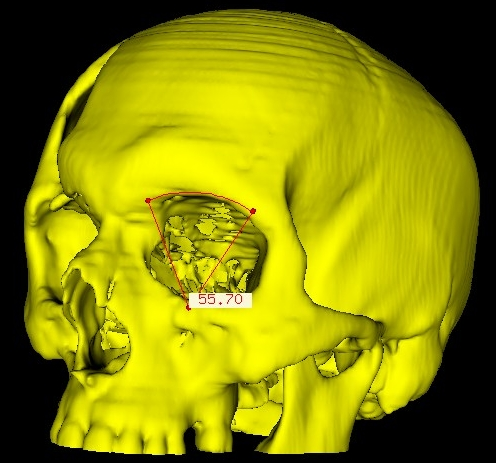
\includegraphics[scale=0.33]{angular_superficie.jpg}
\caption{Angular measurement on surface}
\label{fig:axial_superficie}
\end{figure}

\textbf{Note: Angular measurement is shown in degrees ($^{\circ}$)}


\section{Volumetric Measurement}

Volume and area measurements are made automatically when you create a new surface. These are displayed in the \textbf{Surfaces 3D} tab in the \textbf{Data} management panel, located in the bottom left corner of the screen, as illustrated in Figure~\ref{fig:volumetric_mensure}.

\begin{figure}[!htb]
\centering
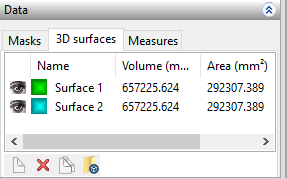
\includegraphics[scale=0.7]{painel_volumetric_measures_en.png}
\caption{Volumetric measurements}
\label{fig:volumetric_mensure}
\end{figure}

\textbf{Note: Volume measurement is given in cubic millimeter ($mm^3$), already the one of area in square millimeter ($mm^2$)}